\begin{center}
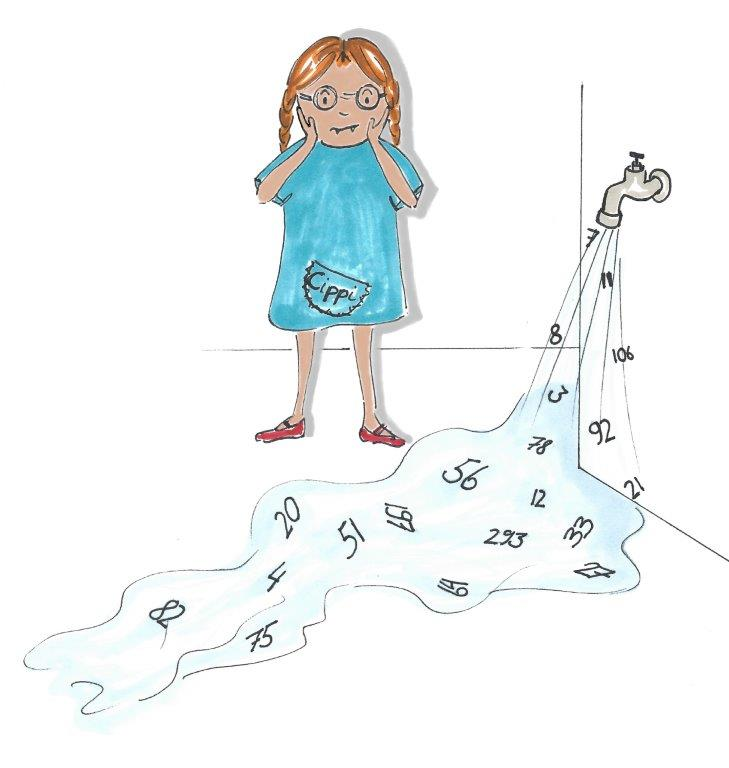
\includegraphics[width=0.4\textwidth]{content/3/chapter7/images/13.png}\\
Cippi在处理数据流
\end{center}

在为无限数据流修改和泛化生成器之前,我想把它作为我们旅程的起点。我有意在源代码中放置了许多输出操作,并且只要求三个值。这种简化和可视化应该有助于理解控制流。

\begin{lstlisting}[style=styleCXX]
// infiniteDataStreamComments.cpp

#include <coroutine>
#include <memory>
#include <iostream>

template<typename T>
struct Generator {
	
	struct promise_type;
	using handle_type = std::coroutine_handle<promise_type>;
	
	Generator(handle_type h): coro(h) {
		std::cout << " Generator::Generator" << '\n';
	}
	handle_type coro;
	
	~Generator() {
		std::cout << " Generator::~Generator" << '\n';
		if ( coro ) coro.destroy();
	}
	Generator(const Generator&) = delete;
	Generator& operator = (const Generator&) = delete;
	Generator(Generator&& oth): coro(oth.coro) {
		oth.coro = nullptr;
	}
	Generator& operator = (Generator&& oth) {
		coro = oth.coro;
		oth.coro = nullptr;
		return *this;
	}
	int getNextValue() {
		std::cout << " Generator::getNextValue" << '\n';
		coro.resume();
		return coro.promise().current_value;
	}
	struct promise_type {
		promise_type() {
			std::cout << " promise_type::promise_type" << '\n';
		}
		
		~promise_type() {
			std::cout << " promise_type::~promise_type" << '\n';
		}
		
		std::suspend_always initial_suspend() {
			std::cout << " promise_type::initial_suspend" << '\n'; \
			
			return {};
		}
		std::suspend_always final_suspend() noexcept {
			std::cout << " promise_type::final_suspend" << '\n';
			return {};
		}
		auto get_return_object() {
			std::cout << " promise_type::get_return_object" << '\n'; \
			
			return Generator{handle_type::from_promise(*this)};
		}
	
		std::suspend_always yield_value(int value) {
			std::cout << " promise_type::yield_value" << '\n'; \
			
			current_value = value;
			return {};
		}
		void return_void() {}
		void unhandled_exception() {
			std::exit(1);
		}
		
		T current_value;
	};
	
};

Generator<int> getNext(int start = 10, int step = 10) {
	std::cout << " getNext: start" << '\n';
	auto value = start;
	while (true) {
		std::cout << " getNext: before co_yield" << '\n';
		co_yield value;
		std::cout << " getNext: after co_yield" << '\n';
		value += step;
	}
}

int main() {
	auto gen = getNext();
	for (int i = 0; i <= 2; ++i) {
		auto val = gen.getNextValue();
		std::cout << "main: " << val << '\n';
	}

}
\end{lstlisting}

可以在\href{https://godbolt.org/z/cTW9Gq}{Compiler Explorer}上执行程序,使控制流更加明显。

\begin{center}
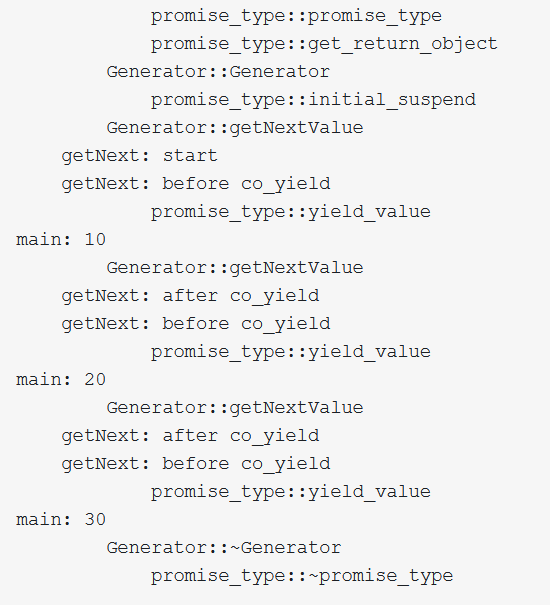
\includegraphics[width=0.5\textwidth]{content/3/chapter7/images/14.png}\\
\end{center}

来分析一下控制流。

调用getNext()(第89行)创建Generator<int>,同时创建promise\_type(第38行),然后下面的get\_return\_object(第55行)创建生成器(第58行),并将其存储在一个局部变量中。当协程第一次挂起时,此调用的结果返回给调用方,初始暂停立即发生(第46行)。因为成员函数调用initial\_suspend返回可等待std::suspend\_always(第46行),控制流继续使用协程getNext,直到指令co\_yield value(第82行)。该调用会映射到yield\_value(int value)(第61行),当前值为current\_value = value(第64行),成员函数yield\_value(int value)返回可等待的std::suspend\_always(第58行)。因此,协程的执行暂停,控制流返回到主函数,for循环开始(第90行)。gen.getNextValue()(第91行)通过使用coro.resume()(第34行)恢复协程来开始执行协程。此外,函数getNextValue()返回使用前面调用的成员函数yield\_value(int value)准备的当前值(第61行)。最后,生成的数字显示在第92行,for循环继续。最后,销毁生成器和promise。

详细分析之后,我想对控制流进行第一次修改。

\subsubsubsection{7.3.1\hspace{0.2cm}修改}

代码段和行号都基于前面的infiniteDataStreamComments.cpp,这里只展示修改部分。

\hspace*{\fill} \\ %插入空行
\noindent
\textbf{7.3.3.1\hspace{0.2cm}协程不会恢复}

当我禁用协程恢复(第91行中的gen.getNextValue())和其值的显示(第92行)时,协程会立即暂停。

\begin{lstlisting}[style=styleCXX]
int main() {
	
	auto gen = getNext();
	for (int i = 0; i <= 2; ++i) {
		// auto val = gen.getNextValue();
		// std::cout << "main: " << val << '\n';
	}

}
\end{lstlisting}

协程永远不会运行。因此,生成器和promise创建后,直接销毁。

\begin{center}
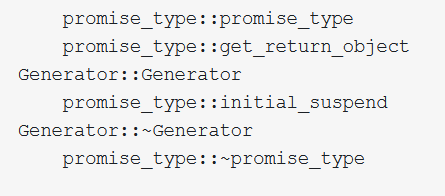
\includegraphics[width=0.5\textwidth]{content/3/chapter7/images/15.png}\\
\end{center}

\hspace*{\fill} \\ %插入空行
\noindent
\textbf{7.3.3.2\hspace{0.2cm}initial\_suspend从不挂起}

在程序中,成员函数initial\_suspend返回可等待的std::suspend\_always(第46行),所以std::suspends\_always会导致协程立即暂停。所以返回std::suspend\_never,而非std::suspend\_always。

\begin{lstlisting}[style=styleCXX]
std::suspend_never initial_suspend() {
	std::cout << " promise_type::initial_suspend" << '\n';
	return {};
}
\end{lstlisting}

从而,协程立即运行,并在函数yield\_value调用时暂停。后续gen.getNextValue()恢复协程,并再次触发成员函数yield\_value的执行。结果会忽略起始值10,所以协程的返回值为20、30和40。

\begin{center}
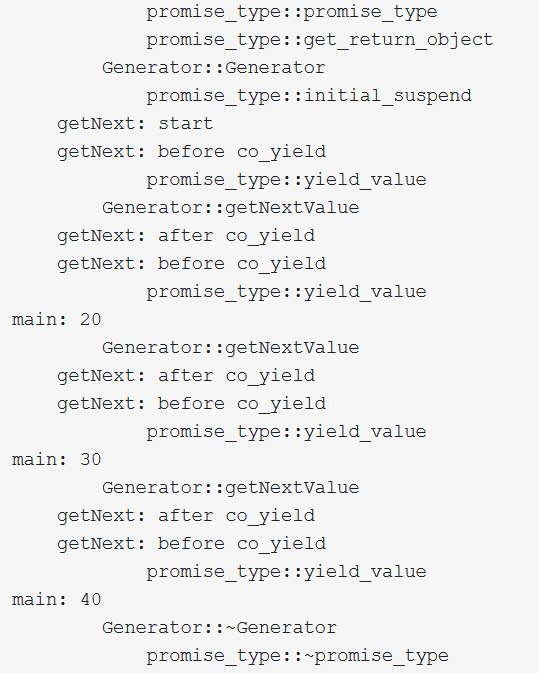
\includegraphics[width=0.5\textwidth]{content/3/chapter7/images/16.png}\\
\end{center}

\hspace*{\fill} \\ %插入空行
\noindent
\textbf{7.3.3.3\hspace{0.2cm}yield\_value从不挂起}

成员函数yield\_value由co\_yield value触发,并准备current\_value。该函数返回std::suspend\_always,因此暂停协程,后续gen.getNextValue必须恢复协程。当我改变成员函数yield\_value的返回值为std::suspend\_never时,来看看会发生什么。

\begin{lstlisting}[style=styleCXX]
std::suspend_never yield_value(int value) {
	std::cout << " promise_type::yield_value" << '\n';
	current_value = value;
	return {};
}
\end{lstlisting}

正如各位猜到的那样,while循环会永远运行,协程不返回任何东西。

\begin{center}
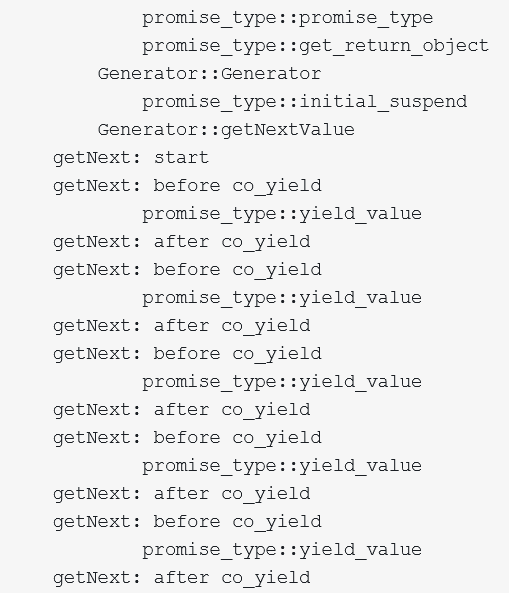
\includegraphics[width=0.5\textwidth]{content/3/chapter7/images/17.png}\\
\end{center}

重构infiniteDataStreamComments.cpp中的生成器很简单,这样它就能产生有限数量的值了。

\subsubsubsection{7.3.2\hspace{0.2cm}泛化}

各位可能会好奇,为什么我从来没有使用Generator的全泛化。现在,我将调整它的实现,以生成标准模板库任意容器的连续元素。

\begin{lstlisting}[style=styleCXX]
// coroutineGetElements.cpp

#include <coroutine>
#include <memory>
#include <iostream>
#include <string>
#include <vector>

template<typename T>
struct Generator {

	struct promise_type;
	using handle_type = std::coroutine_handle<promise_type>;
	
	Generator(handle_type h): coro(h) {}
	
	handle_type coro;
	
	~Generator() {
		if ( coro ) coro.destroy();
	}
	Generator(const Generator&) = delete;
	Generator& operator = (const Generator&) = delete;
	Generator(Generator&& oth): coro(oth.coro) {
		oth.coro = nullptr;
	}
	Generator& operator = (Generator&& oth) {
		coro = oth.coro;
		oth.coro = nullptr;
		return *this;
	}
	T getNextValue() {
		coro.resume();
		return coro.promise().current_value;
	}
	struct promise_type {
		promise_type() {}
		
		~promise_type() {}
		
		std::suspend_always initial_suspend() {
			return {};
		}
		std::suspend_always final_suspend() noexcept {
			return {};
		}
		auto get_return_object() {
			return Generator{handle_type::from_promise(*this)};
		}
		
		std::suspend_always yield_value(const T value) {
			current_value = value;
			return {};
		}
		void return_void() {}
		void unhandled_exception() {
			std::exit(1);
		}
		
		T current_value;
	};

};

template <typename Cont>
Generator<typename Cont::value_type> getNext(Cont cont) {
	for (auto c: cont) co_yield c;
}

int main() {

	std::cout << '\n';
	
	std::string helloWorld = "Hello world";
	auto gen = getNext(helloWorld);
	for (int i = 0; i < helloWorld.size(); ++i) {
		std::cout << gen.getNextValue() << " ";
	}
	
	std::cout << "\n\n";
	
	auto gen2 = getNext(helloWorld);
	for (int i = 0; i < 5 ; ++i) {
		std::cout << gen2.getNextValue() << " ";
	}
	
	std::cout << "\n\n";
	
	std::vector myVec{1, 2, 3, 4 ,5};
	auto gen3 = getNext(myVec);
	for (int i = 0; i < myVec.size() ; ++i) {
		std::cout << gen3.getNextValue() << " ";
	}
	
	std::cout << '\n';

}
\end{lstlisting}

本例中,生成器进行了实例化,并使用了三次。前两种情况下,gen(第75行)和gen2(第82行)使用std::string helloWorld进行了初始化,而gen3使用std::vector<int>(第90行)进行初始化。程序的输出应该没啥好说的。第77行依次返回字符串helloWorld的所有字符,第84行只返回前5个字符,第92行返回std::vector<int>的元素。

您可以在\href{https://godbolt.org/z/j9znva}{Compiler Explorer}上尝试编译运行该程序。

\begin{tcblisting}{commandshell={}}
H e l l o  w o r l d

H e l l o

1 2 3 4 5
\end{tcblisting}

简而言之,Generator<T>的实现几乎与前一个示例完全相同。与前一个示例的关键区别是协程getNext。

\begin{lstlisting}[style=styleCXX]
template <typename Cont>
Generator<typename Cont::value_type> getNext(Cont cont) {
	for (auto c: cont) co_yield c;
}
\end{lstlisting}

getNext是一个函数模板,接受容器作为参数,并在基于范围的for循环中遍历容器的所有元素。每次迭代后,函数模板都会暂停。生成器的返回类型可能会让你感到惊讶,Cont::value\_type是一个依赖的模板参数,解析器需要对此进行提示。默认情况下,若可以解释为类型或非类型,则编译器假定其是一个非类型。出于这个原因,必须把typename放在Cont::value\_type的前面。


\newpage












